\documentclass[conference]{IEEEtran}
\usepackage{cite}
\usepackage{amsmath,amssymb,amsfonts}
\usepackage{graphicx}
\usepackage{textcomp}
\usepackage{booktabs}
\usepackage{array}
\usepackage[hidelinks]{hyperref}
\usepackage{balance}

\renewcommand\IEEEkeywordsname{Keywords}

\begin{document}

\title{Benchmarking Multi-View Tree-Level Oil Palm Bunch Counting Under a Fixed Detector}

\author{
\IEEEauthorblockN{Muhammad Zainal Muttaqin\IEEEauthorrefmark{1},
Fatma Indriani\IEEEauthorrefmark{1},
Setyo Wahyu Saputro\IEEEauthorrefmark{1},
Alia Rahmi\IEEEauthorrefmark{2},\\
Dwi Kartini\IEEEauthorrefmark{1},
Triando Hamonangan Saragih\IEEEauthorrefmark{1},
Naufal Said\IEEEauthorrefmark{1} and
Hartoni\IEEEauthorrefmark{3}}
\IEEEauthorblockA{\IEEEauthorrefmark{1}\textit{Department of Computer Science,}\\
\textit{Faculty of Mathematics and Natural Sciences,}\\
\textit{Lambung Mangkurat University,} Banjarbaru, Indonesia\\
f.indriani@ulm.ac.id}
\IEEEauthorblockA{\IEEEauthorrefmark{2}\textit{Department of Agro-Industrial Technology,}\\
\textit{Faculty of Agriculture, Lambung Mangkurat University,}\\
Banjarbaru, Indonesia}
\IEEEauthorblockA{\IEEEauthorrefmark{3}\textit{Department of Agribusiness,}\\
\textit{Faculty of Agriculture, Lambung Mangkurat University,}\\
Banjarbaru, Indonesia}
}

\maketitle

\begin{abstract}
\bfseries Tree-level yield forecasting often requires a count of objects in several
readiness classes rather than a single total. Multi-view imaging helps recover
objects hidden by occlusion, but it also creates duplicate observations of the
same physical object across views. A deployed system must therefore solve
detection and tree-level aggregation jointly. Whether failures arise from the
detector or the aggregation step has not been isolated by prior work. This paper
benchmarks that question on 953 oil palm trees and 3,992 side-view images under
two detection conditions. The benchmark evaluates five regression counters under
both conditions and ablates eight feature configurations in the fixed-detector
setting. When the counting model receives annotated detections, it reaches
98.05\% accuracy at the class level and 92.20\% at the whole-tree level. When
the same task uses outputs from a fixed detector (YOLO26m), those accuracies drop to
77.48\% and 32.62\%. The 20.57 percentage-point gap remains after testing all
model and feature combinations. This indicates detector quality is the limiting
factor, not the tree-level counting step.
\end{abstract}

\begin{IEEEkeywords}
\bfseries\itshape Oil palm, fresh fruit bunch, black bunch census, multi-view counting, object
detection, YOLO, tree-level regression, agricultural computer vision.
\end{IEEEkeywords}

% ---------------------------------------------------------------------------
\section{Introduction}
% ---------------------------------------------------------------------------

Harvest scheduling in commercial oil palm plantations depends on knowing, for
every tree, how many fruit bunches belong to each operational maturity class.
The Black Bunch Census (BBC) formalises this requirement into a four-class count
vector, B1 through B4, where each class carries distinct timing and logistics
implications~\cite{ref12}. Automating BBC through image-based counting would
reduce the cost and subjectivity of manual field surveys. The central
operational requirement is reproducing the per-class disaggregation rather than
collapsing it into a single total.

Tree-level counting is geometrically harder than image-level
detection~\cite{ref1}. Bunches surround the full circumference of an oil palm,
so a single image misses bunches due to occlusion, viewing angle, or overlapping
fronds. Multi-view acquisition reduces missed bunches by photographing each tree
from four to eight side views, but the same physical bunch then appears in
several images. Fig.~\ref{fig:crossview} illustrates the effect: a single B3
bunch is visible in three adjacent side views of the same tree. Naive summation
of per-image detections counts appearances rather than bunch identities and is
biased upward on this dataset.

\begin{figure*}[!t]
  \centering
  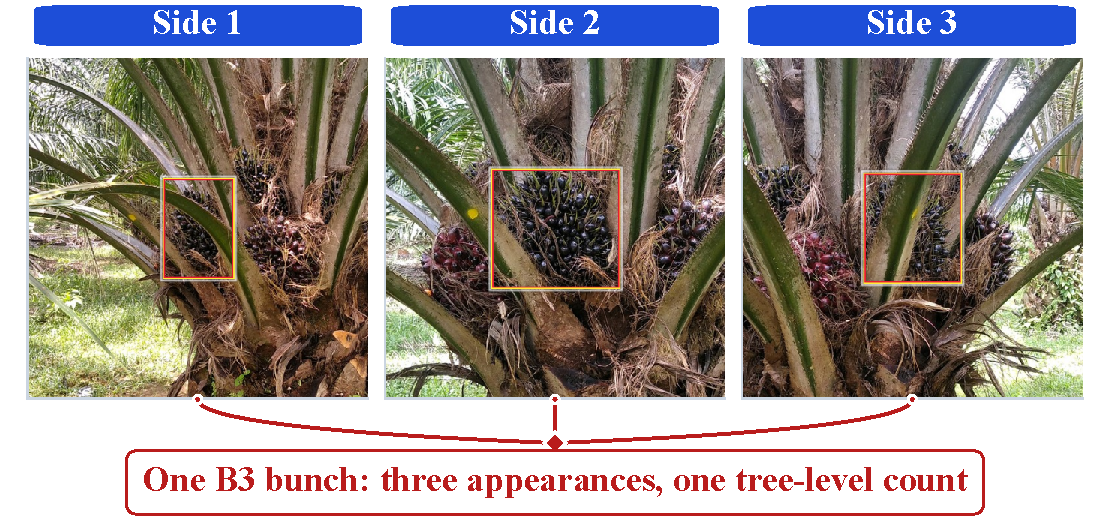
\includegraphics[width=\textwidth]{../figures/paper/fig01_cross_view_linking.pdf}
  \caption{A single physical B3 bunch is visible across three adjacent side
  views. If every per-image detection is counted, three appearances are added
  for one bunch. Tree-level counting must therefore aggregate evidence across
  views rather than sum it.}
  \label{fig:crossview}
\end{figure*}

Multi-view deduplication has been studied across several crops through geometric
fusion, sequential scan, and neural reconstruction. Mango counting systems
associated detections across sequential passes using navigation data and canopy
geometry~\cite{ref5}, and apple pipelines built row-level maps from overlapping
two-side scans~\cite{ref6}. Comparative evaluation of multi-view apple pipelines
shows that counting errors typically originate in detection quality rather than
the aggregation step~\cite{ref7}. Sparse and calibrated viewpoints have been
addressed through correspondence-free triangulation~\cite{ref3} and few-view 3D
reconstruction~\cite{ref4}, and recent neural-field methods count from
unstructured photographs in a shared 3D representation~\cite{ref8}. Most of
these systems depend on dense sequential overlap, a moving sensor platform, or
calibrated geometry, and none isolates detector quality from counter quality as
separate error sources.

Regression-based aggregation maps detection statistics to a tree-level count
vector, an approach well established in agricultural
vision~\cite{ref1,ref6,ref7}. YOLO-style single-stage detectors are now the
standard front-end for such pipelines~\cite{ref14,ref15}. The regressor is
typically evaluated only on the detector outputs available during the study,
so detector quality and counter quality enter the accuracy estimate jointly.
When end-to-end performance falls short, this coupling makes it impossible to
determine whether effort should target the detector or the counter. Isolating
the two contributions requires evaluating the same counting model under both
controlled and realistic detection conditions.

Oil palm counting has received less systematic study than apple or mango.
Detectors for fresh fruit bunches (FFB) and maturity classification have
reached production-level accuracy on ripe bunches but show recurring weaknesses
on partially occluded and maturity-ambiguous classes~\cite{refNaftali2024},
with both two-stage and YOLO-style architectures explored~\cite{ref9,ref10,ref11,ref13}. The closest public oil palm resource is a video dataset annotated at the frame level for
detection~\cite{refSuharjito2025}. Tree-level counting labels are absent, and
no counting evaluation has been reported on it. No existing benchmark evaluates
tree-level counting strategies under controlled detection conditions or separates
detector error from counter error for this task.

This paper closes that gap by benchmarking tree-level multi-view BBC counting
under two detection conditions on the SawitMVC dataset (953 trees, 3,992
images)~\cite{refIndriani2026}. The first condition uses ground-truth detections to isolate counter
performance from detector error, and the second uses a fixed YOLO26m detector
to reflect a realistic deployed pipeline. Five regression models and eight
feature configurations are evaluated within each condition. The paper makes
three contributions: (1) a systematic benchmark of tree-level bunch counting
under two detection conditions, establishing an accuracy ceiling and a
deployment baseline on the same dataset; (2) a feature ablation study showing
that enriched feature representations recover only a marginal fraction of the
detector-driven gap; and (3) evidence that the primary performance bottleneck
is detector output quality rather than the choice of counting model.

% ---------------------------------------------------------------------------
\section{Methodology}
% ---------------------------------------------------------------------------

\subsection{Dataset and Task Definition}
\label{sec:task}

The benchmark uses the SawitMVC multi-view dataset: 953 oil palm trees,
3,992 side-view images, four maturity classes (B1, B2, B3, and B4), and 4 to
8 side views per tree. The fixed split contains 716 training trees, 96
validation trees, and 141 test trees. Dataset construction, annotation
protocol, and per-class composition are documented in~\cite{refIndriani2026}.

For tree $i$, the ground-truth target is the count vector
\begin{equation}
  \mathbf{y}_i = [\,y_{i,B1},\;y_{i,B2},\;y_{i,B3},\;y_{i,B4}\,],
\end{equation}
and the prediction is $\hat{\mathbf{y}}_i =
[\,\hat{y}_{i,B1},\ldots,\hat{y}_{i,B4}\,]$. The evaluation unit is the tree,
not the individual image: per-image appearance counts are not valid BBC outputs.

Let $a_{i,c}$ denote the number of detected appearances of class $c$ across
all views of tree $i$. The naive multi-view estimator
\begin{equation}
  \hat{y}_{i,c}^{\text{naive}} = a_{i,c}
\end{equation}
is biased upward whenever a bunch is visible from more than one side. Under GT
annotations, this estimator reaches only 50.00\% Class $\pm$1 Acc and 6.38\%
Tree $\pm$1 Acc on the test split, which motivates learned tree-level
aggregation rather than direct summation.

\subsection{Detection Conditions}

The benchmark isolates detector error from counter error by evaluating the same
counters under two detection conditions, illustrated in
Fig.~\ref{fig:conditions}.

\begin{figure}[!htbp]
  \centering
  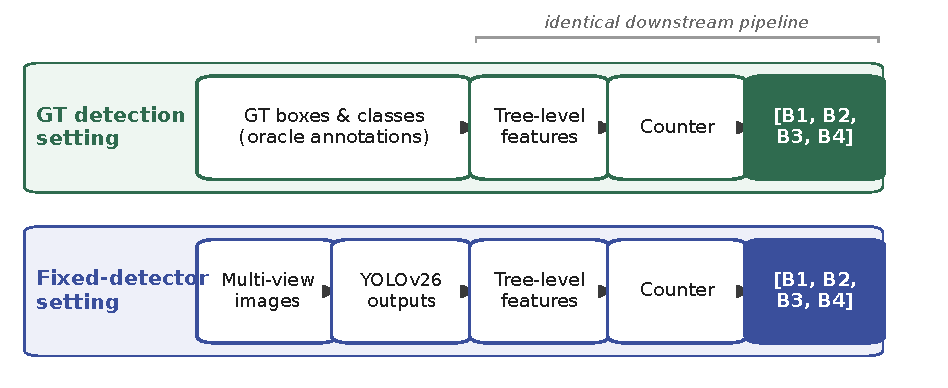
\includegraphics[width=\columnwidth]{../figures/paper/fig02_detection_conditions.pdf}
  \caption{Two detection conditions used in the benchmark. \textit{Top:} the
  GT detection setting supplies ground-truth boxes and classes to the
  tree-level feature extractor, so detector output quality is removed as an
  error source. \textit{Bottom:} the fixed-detector setting supplies cached
  YOLO26m outputs, so detector misses and class confusions enter the
  pipeline before counting.}
  \label{fig:conditions}
\end{figure}

In the \textit{GT detection setting}, the feature extractor reads ground-truth
bounding boxes and classes directly from the annotation files. Counters trained
on these features upper-bound how well a tree-level counter can perform when
detections are accurate. In the \textit{fixed-detector setting}, the feature
extractor reads cached YOLO26m~\cite{ref15} predictions from the released
\texttt{y26mv2} checkpoint. The detector was trained on the official 716-tree training
split for 60 epochs (batch size 32, image size 640, patience 60, seed 42).
Inference uses the repository default confidence threshold of 0.25 and the
standard Ultralytics post-processing settings. A single detector checkpoint is
used for all counter and feature configurations, so any observed differences
come from the counter or feature representation rather than detector retraining.
Preliminary experiments across multiple detector architectures and training
configurations produced no meaningful performance differences on this dataset,
indicating that the bottleneck lies in task difficulty rather than detector
design. The y26mv2 checkpoint was therefore selected as a representative fixed
detector. A deeper detector study, including alternative architectures and
depth-augmented inputs, is planned as future work.

\begin{table}[!htbp]
  \centering
  \footnotesize
  \setlength{\tabcolsep}{4pt}
  \caption{YOLO26m validation detection performance, reported under the
    COCO mAP50 convention~\cite{ref16}.}
  \label{tab:yolo}
  \begin{tabular}{@{}lrr@{}}
    \toprule
    Class   & mAP50          & Recall         \\
    \midrule
    B1      & \textbf{0.746} & \textbf{0.801} \\
    B2      & 0.425          & 0.433          \\
    B3      & 0.550          & 0.656          \\
    B4      & 0.363          & 0.389          \\
    Overall & 0.521          & 0.570          \\
    \bottomrule
  \end{tabular}
\end{table}

The per-class weakness on B4 and the moderate recall on B3 in
Table~\ref{tab:yolo} are revisited in Section~\ref{sec:gap}.

\subsection{Feature Vectors}

Given either set of detections, observations from all views of a tree are
aggregated into a fixed-length feature vector. The 13-dimensional baseline
$F_0$ contains, for each class $c$, the total count $s_c$, the per-side
maximum $m_c$, and the per-side mean $\mu_c$, plus the number of available
views $n_{\text{views}}$:
\begin{equation}
  F_0 = [\,s_{B1\text{:}B4},\;m_{B1\text{:}B4},\;\mu_{B1\text{:}B4},\;
        n_{\text{views}}\,].
\end{equation}

Three optional groups extend $F_0$. The confidence group (20-dim) contains
five per-class statistics: confidence sum, mean, max, count above 0.5, and
count above 0.6. Spatial position provides a separate signal: the mean
normalized vertical centroid $\overline{cy}_c$ and mean bounding-box area
$\overline{A}_c$ for each class form an 8-dimensional group that reflects the
vertical separation of maturity classes on the tree. A 20-dimensional
side-distribution group records per-side std, per-side min, coefficient of
variation, number of sides with detections, and a consistency score for each
class.

A cross-class composition group (6-dim), consisting of the total detection
count, four class fractions, and a B3-vs-(B2+B3) mixture ratio, completes the
67-dimensional combined set $F_{\text{all}}$:
\begin{equation*}
  F_{\text{all}} = F_0 \cup \text{conf} \cup \text{spatial}
                      \cup \text{distrib} \cup \text{composition}.
\end{equation*}

Eight feature sets are evaluated: $F_0$, $F_0$+conf, $F_0$+spatial,
$F_0$+distrib, $F_0$+conf+spatial, $F_0$+conf+distrib, $F_0$+distrib+spatial,
and $F_{\text{all}}$.

\subsection{Counter Models and Evaluation Metrics}

Three heuristic baselines are included as reference points. The \textit{naive
sum} sums all detected appearances per class (defined in
Section~\ref{sec:task}). The \textit{global divisor} scales the naive sum by
a fixed constant $k$ fit to the training split, correcting for the average
number of times a single bunch is observed across views. The
\textit{visibility-adaptive divisor} replaces the global constant with a
per-tree factor that varies with the number of side views captured for that
tree.

Five regression models are evaluated in both detection conditions: Linear
Regression, Ridge~\cite{ref19}, ElasticNet~\cite{ref17}, SVM~\cite{ref20}, and
Random Forest~\cite{ref18}. Each counter maps a tree feature vector
$\mathbf{x}_i$ to the count vector $\hat{\mathbf{y}}_i =
f_{\theta}(\mathbf{x}_i)$.

All counter models are trained on the 716-tree training split and evaluated on
the fixed 141-tree test split. Class-level $\pm 1$ correctness for tree $i$
and class $c$ is
\begin{equation}
  I_{i,c}^{\pm 1} =
  \begin{cases}
    1, & |\hat{y}_{i,c} - y_{i,c}| \leq 1, \\
    0, & \text{otherwise}.
  \end{cases}
\end{equation}

\textbf{Class $\pm$1 Acc} averages this indicator over all test trees and
classes:
\begin{equation}
  \text{Class } \pm 1 \text{ Acc} =
    \frac{1}{4N}\sum_{i=1}^{N}\sum_{c=1}^{4} I_{i,c}^{\pm 1}.
\end{equation}

\textbf{Tree $\pm$1 Acc} is stricter: a tree counts as correct only if all
four class predictions are within $\pm 1$ simultaneously,
\begin{equation}
  \text{Tree } \pm 1 \text{ Acc} =
    \frac{1}{N}\sum_{i=1}^{N}
      \mathbb{1}\!\left(\sum_{c=1}^{4} I_{i,c}^{\pm 1} = 4\right).
\end{equation}

\textbf{Macro MAE} is the mean absolute error averaged over trees and classes.
\textbf{Signed class bias} is the per-class mean $\hat{y}_{i,c} - y_{i,c}$;
positive values indicate over-counting, negative values under-counting. Bias
is reported alongside accuracy because operational aggregate yield estimates
are sensitive to directional error rather than absolute error alone.\footnote{Source code: \url{https://github.com/ULM-SawitMVC/Baseline-SawitMVC}.}

% ---------------------------------------------------------------------------
\section{Results and Discussion}
% ---------------------------------------------------------------------------

The results follow the detector-counter question directly. Section~\ref{sec:gt}
estimates the counter ceiling under GT detections, Section~\ref{sec:fixed}
measures the deployed fixed-detector setting, Section~\ref{sec:ablation} tests
whether richer features recover the loss, and Section~\ref{sec:gap} compares
the two conditions per class.

\subsection{GT Detection Setting}
\label{sec:gt}

Table~\ref{tab:gt} reports counting results when the counter receives GT
detections. Naive appearance summation yields only 50.00\% Class $\pm$1 Acc
and 6.38\% Tree $\pm$1 Acc. This confirms that duplicate visibility cannot be
ignored and that direct summation is not a viable estimator. The global divisor
and visibility-adaptive divisor recover most of the loss, and ElasticNet
improves further to 98.05\% Class $\pm$1 Acc. Under accurate detections, the
remaining counting problem is therefore simple enough for compact regression
models.

\begin{table}[!htbp]
  \centering
  \scriptsize
  \setlength{\tabcolsep}{2.3pt}
  \caption{Counting under the GT detection setting on the 141-tree test split.}
  \label{tab:gt}
  \begin{tabular}{@{}lcrrr@{}}
    \toprule
    Method                      & Type  & Class $\pm$1 & Tree $\pm$1 & MAE            \\
    \midrule
    Naive sum                   & Heur. & 50.00\%          &  6.38\%     & 2.142          \\
    Global divisor              & Heur. & 95.39\%          & 85.11\%     & 0.376          \\
    Visibility-adapt. divisor   & Heur. & 95.92\%          & 87.23\%     & 0.340          \\
    ElasticNet                  & ML    & \textbf{98.05\%} & \textbf{92.20\%} & 0.277      \\
    SVM                         & ML    & 97.87\%          & 91.49\%     & \textbf{0.266} \\
    Ridge                       & ML    & 97.70\%          & 90.78\%     & 0.275          \\
    Linear reg.                 & ML    & 97.52\%          & 90.07\%     & 0.277          \\
    Random forest               & ML    & 95.92\%          & 84.40\%     & 0.365          \\
    \bottomrule
  \end{tabular}
\end{table}

The four best machine-learning counters (ElasticNet, SVM, Ridge, LR) sit within
0.5 percentage points of each other on Class $\pm$1 Acc and within 2.2 points
on Tree $\pm$1 Acc. Random Forest is the only counter that underperforms in this
setting. This narrow spread indicates that, when detector evidence is accurate,
the choice among standard counter families is not the limiting factor.

\subsection{Fixed-Detector Setting}
\label{sec:fixed}

Moving from GT to cached YOLO26m detections, the best $F_0$ result
(ElasticNet, 76.42\% Class $\pm$1 Acc) trails the same counter under GT by
more than 20 percentage points (Table~\ref{tab:fixed}). All five counters
remain within a 3.2 percentage-point window on Class $\pm$1 Acc. The large
drop across the two detection conditions, coupled with the small spread among
counters, points to the detector output rather than the counter family as the
main source of loss.

\begin{table}[!htbp]
  \centering
  \footnotesize
  \setlength{\tabcolsep}{3pt}
  \caption{Fixed-detector counting with F0 features on the 141-tree test split.}
  \label{tab:fixed}
  \begin{tabular}{@{}lrrr@{}}
    \toprule
    Counter           & Class $\pm$1 Acc & Tree $\pm$1 Acc  & Macro MAE      \\
    \midrule
    ElasticNet        & \textbf{76.42\%} & 29.79\%          & \textbf{1.043} \\
    Ridge             & 76.06\%          & 28.37\%          & 1.053          \\
    Linear Regression & 75.71\%          & \textbf{30.50\%} & 1.048          \\
    SVM               & 74.82\%          & 29.08\%          & \textbf{1.043} \\
    Random Forest     & 73.23\%          & 26.95\%          & 1.110          \\
    \bottomrule
  \end{tabular}
\end{table}

The per-class breakdown in Table~\ref{tab:perclass} shows that B1 stays near
its GT ceiling while B3 falls to 55--56\% Class $\pm$1 Acc across all five
counters. B2 and B4 sit at intermediate losses. This profile matches the
detection recall in Table~\ref{tab:yolo}: the weakest detector classes lose the
most counting accuracy.

\begin{table}[!htbp]
  \centering
  \scriptsize
  \setlength{\tabcolsep}{3pt}
  \caption{Per-class Class $\pm$1 Acc of fixed-detector counters with F0
    features on the 141-tree test split.}
  \label{tab:perclass}
  \begin{tabular}{@{}lrrrr@{}}
    \toprule
    Counter           & B1               & B2               & B3               & B4               \\
    \midrule
    ElasticNet        & \textbf{96.45\%} & \textbf{80.14\%} & \textbf{56.03\%} & \textbf{73.05\%} \\
    Ridge             & 95.74\%          & \textbf{80.14\%} & \textbf{56.03\%} & 72.34\%          \\
    Linear Regression & \textbf{96.45\%} & 79.43\%          & 55.32\%          & 71.63\%          \\
    SVM               & 95.74\%          & 76.60\%          & 55.32\%          & 71.63\%          \\
    Random Forest     & 95.74\%          & 73.76\%          & \textbf{56.03\%} & 67.38\%          \\
    \bottomrule
  \end{tabular}
\end{table}

\subsection{Feature Ablation}
\label{sec:ablation}

\begin{table}[!htbp]
  \centering
  \scriptsize
  \setlength{\tabcolsep}{2.2pt}
  \caption{Ridge feature ablation in the fixed-detector setting.}
  \label{tab:ablation}
  \begin{tabular}{@{}>{\raggedright\arraybackslash}p{0.39\columnwidth}rrrr@{}}
    \toprule
    Features                            & Dim & Class $\pm$1 & Tree $\pm$1 & MAE            \\
    \midrule
    $F_0$                                  &  13 & 76.06\%          & 28.37\%          & 1.053          \\
    $F_0$ + confidence                     &  33 & 75.89\%          & 29.79\%          & 1.059          \\
    $F_0$ + spatial                        &  21 & 76.60\%          & 30.50\%          & 1.046          \\
    $F_0$ + side-distribution              &  33 & 74.82\%          & 28.37\%          & 1.060          \\
    $F_0$ + confidence + spatial           &  41 & 76.24\%          & 29.08\%          & 1.059          \\
    $F_0$ + confidence + side-distribution &  53 & 76.42\%          & 29.79\%          & 1.060          \\
    $F_0$ + side-distribution + spatial    &  41 & 75.71\%          & 30.50\%          & 1.048          \\
    $F_{\text{all}}$                    &  67 & \textbf{77.48\%} & \textbf{32.62\%} & \textbf{1.035} \\
    \bottomrule
  \end{tabular}
\end{table}

Whether enriched features can recover the detector-driven gap is tested by
fixing Ridge and varying the feature configuration (Table~\ref{tab:ablation}).
$F_0$ starts at 76.06\% Class $\pm$1 Acc. Spatial features alone raise this to
76.60\%; the vertical centroid and bounding-box area encode residual maturity
position that the raw count statistics in $F_0$ do not capture directly.
Confidence features do not improve the baseline individually, and adding
side-distribution alone reduces Class $\pm$1 Acc to 74.82\%, below the $F_0$
baseline, suggesting this group introduces noise under the current detector.

The full $F_{\text{all}}$ set gives the best ablation result at 77.48\% Class
$\pm$1 Acc and 32.62\% Tree $\pm$1 Acc. The gain over $F_0$ is 1.42 percentage
points at class level and 4.25 points at tree level. This 1.42-pp gain is the
ceiling of feature-side improvement. The best feature set narrows only a small
fraction of the gap between GT and fixed-detector conditions.

\subsection{GT vs.\ Fixed-Detector Gap}
\label{sec:gap}

The central comparison is the per-class gap between ideal detections and the
fixed detector, shown with the signed bias of the best configuration in
Fig.~\ref{fig:gap}.

\begin{figure}[!htbp]
  \centering
  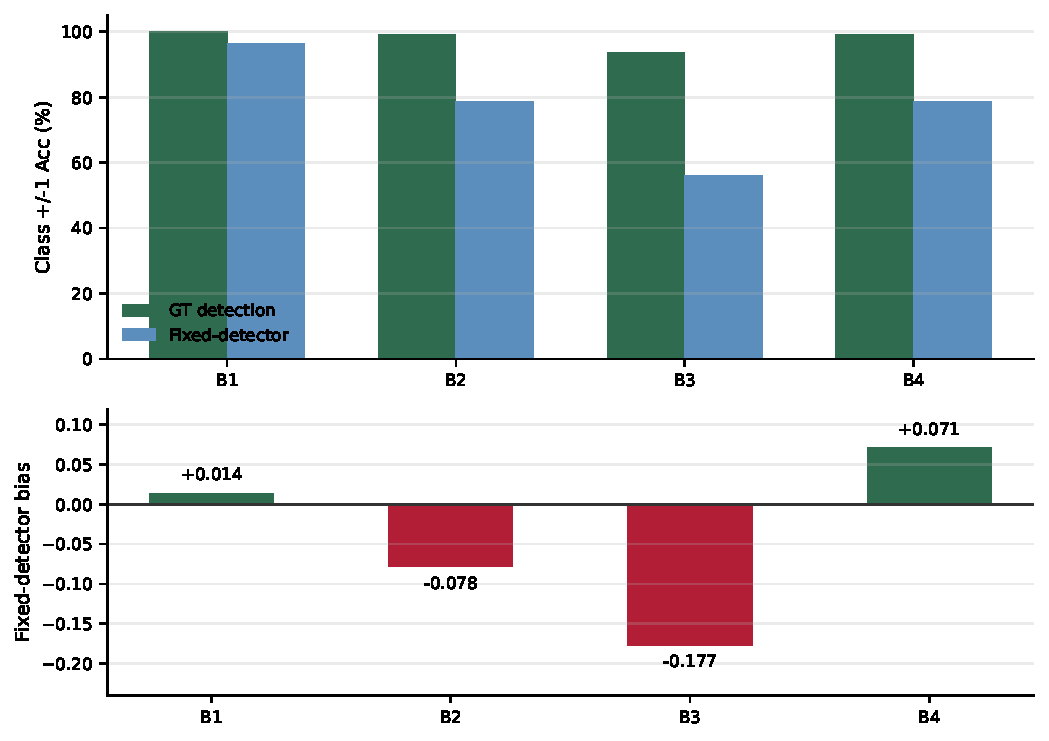
\includegraphics[width=\columnwidth]{../figures/paper/fig03_gap_bias.pdf}
  \caption{\textit{Top:} Per-class Class $\pm$1 Acc for the best counter in
  each detection condition (ElasticNet under GT; Ridge + $F_{\text{all}}$ under
  the fixed detector). Counting is near ceiling under GT detection but drops
  sharply under the fixed detector. \textit{Bottom:} Per-class signed bias of
  Ridge + $F_{\text{all}}$ in the fixed-detector setting. Negative values
  indicate systematic under-counting; the under-count is concentrated on B2
  and especially B3.}
  \label{fig:gap}
\end{figure}

The absolute gap is large, at 20.57 percentage points in Class $\pm$1 Acc and
59.58 percentage points in Tree $\pm$1 Acc, as summarized in
Table~\ref{tab:summary}. The loss is not uniform across maturity classes. B1
loses only $\approx$2.8\,pp between the two conditions, while B2 loses
$\approx$16.3\,pp, B3 loses 36.2\,pp, and B4 loses $\approx$27.0\,pp. This
profile aligns with Table~\ref{tab:yolo}, where B3 and B4 have weaker detector
recall and fall furthest below the GT ceiling.

The bias plot adds direction to the accuracy gap. The fixed-detector Ridge +
$F_{\text{all}}$ pipeline under-counts B2 by 0.078 and B3 by 0.177 bunches per
tree on average. Because plantation-level forecasts aggregate per-tree
predictions across blocks, systematic under-counting in B2 and B3 would carry
into the next-cycle harvest estimate rather than cancel out as random noise.

\begin{table}[!htbp]
  \centering
  \scriptsize
  \setlength{\tabcolsep}{2.4pt}
  \caption{Consolidated test-set summary. Biases are ordered by class.}
  \label{tab:summary}
  \begin{tabular}{@{}>{\raggedright\arraybackslash}p{0.27\columnwidth}rrrrrr@{}}
    \toprule
    Config & Class $\pm$1 & Tree $\pm$1 & B1 & B2 & B3 & B4 \\
    \midrule
    GT, ElasticNet &
      98.05\% & 92.20\% & $-.050$ & $+.043$ & $-.064$ & $-.028$ \\
    Fixed, Ridge + $F_{\text{all}}$ &
      77.48\% & 32.62\% & $+.014$ & $-.078$ & $-.177$ & $+.071$ \\
    \bottomrule
  \end{tabular}
\end{table}

Across all counter and feature combinations, the per-class gap traces the
detector recall profile in Table~\ref{tab:yolo}, not the spread among counter
families. Multi-view duplicate visibility is real and large, but learned
tree-level counters handle it when detector evidence is accurate
(Section~\ref{sec:gt}). Once a fixed detector replaces ground-truth boxes,
counter performance drops sharply (Section~\ref{sec:fixed}), and richer
features or different counter families close only a small fraction of the loss
(Section~\ref{sec:ablation}). This aligns with the finding in~\cite{ref7} that
counting errors typically trace to detection quality. The present benchmark puts
a concrete upper bound on what counter-side improvements can contribute.

These findings have a direct consequence for system design. The gap between the
GT ceiling and the fixed-detector result sets an upper bound on what counter-side
changes alone can recover. No counter or feature combination tested here narrows
that gap by more than 1.42 pp at the class level. Improving detector recall on
B3 and B4, the two weakest classes, is therefore the highest-leverage
intervention available in this pipeline.

Several limitations bound the scope of these findings. The benchmark uses a
single dataset of 953 trees from two plantations in South Kalimantan, so
absolute numbers may shift under other regions, varieties, or acquisition
protocols. Only one detector checkpoint (YOLO26m) is tested, and a different
detector family could change the per-class error profile. The tree-level
counters treat each tree independently and ignore plantation-scale spatial or
temporal regularities that operational forecasts sometimes exploit. The
four-class B1 through B4 taxonomy also admits visual ambiguity at the B2/B3 and
B3/B4 boundaries. Future work should prioritize B3/B4 recall, confidence
calibration for counting, and explicit cross-view association or geometry-aware
aggregation~\cite{ref2,ref3,ref4} rather than expanding the tree-level feature
set further.

% ---------------------------------------------------------------------------
\section{Conclusion}
% ---------------------------------------------------------------------------

This paper benchmarks multi-view tree-level oil palm FFB counting by evaluating
the same counters under GT detections and cached YOLO26m outputs. With GT
detections, standard regression counters achieve near-ceiling accuracy on the
B1 through B4 count. With the fixed detector, neither additional feature groups
nor alternative counter families narrow the gap appreciably. On SawitMVC under
this detector checkpoint, the limiting factor is detector output quality,
especially for B3 and B4, rather than the choice among the tested tree-level
counters. Closing the gap will require improving the detector, not the counter.

% ---------------------------------------------------------------------------
\section*{Acknowledgment}
% ---------------------------------------------------------------------------

This research was funded by the Badan Pengelola Dana Perkebunan (BPDP),
Indonesia, under contract number PRJ-36/BPDP/2026, through Universitas Lambung
Mangkurat (ULM), Banjarmasin, Indonesia.

% ---------------------------------------------------------------------------
\balance
\begin{thebibliography}{00}

\bibitem{ref12}
M.~Kerstan and T.~Fairhurst,
``Use of OMP for accurate crop forecasts,''
Agrisoft Systems and Tropical Crop Consultants Limited. [Online]. Available:
\url{https://www.agrisoft-systems.com/wp-content/uploads/Papers/CropForecastsWithOMPBBC.pdf}.
[Accessed: May 2026].

\bibitem{ref1}
A.~Koirala, K.~B.~Walsh, Z.~Wang, and C.~McCarthy,
``Deep learning: method overview and review of use for fruit detection and
yield estimation,''
\textit{Computers and Electronics in Agriculture}, vol.~162, pp.~219--234,
Jul.~2019, doi: \url{https://doi.org/10.1016/j.compag.2019.04.017}.

\bibitem{ref5}
M.~Stein, S.~Bargoti, and J.~Underwood,
``Image based mango fruit detection, localisation and yield estimation using
multiple view geometry,''
\textit{Sensors}, vol.~16, no.~11, Art. no.~1915, Nov.~2016,
doi: \url{https://doi.org/10.3390/s16111915}.

\bibitem{ref6}
P.~Roy, A.~Kislay, P.~A.~Plonski, J.~Luby, and V.~Isler,
``Vision-based preharvest yield mapping for apple orchards,''
\textit{Computers and Electronics in Agriculture}, vol.~164, Art. no.~104897,
Sep.~2019, doi: \url{https://doi.org/10.1016/j.compag.2019.104897}.

\bibitem{ref7}
N.~H\"{a}ni, P.~Roy, and V.~Isler,
``A comparative study of fruit detection and counting methods for yield
mapping in apple orchards,''
\textit{Journal of Field Robotics}, vol.~37, no.~2, pp.~263--282, Mar.~2020,
doi: \url{https://doi.org/10.1002/rob.21902}.

\bibitem{ref3}
M.~Gaillard, B.~Benes, M.~C.~Tross, and J.~C.~Schnable,
``Multi-view triangulation without correspondences,''
\textit{Computers and Electronics in Agriculture}, vol.~206, Art. no.~107688,
Mar.~2023, doi: \url{https://doi.org/10.1016/j.compag.2023.107688}.

\bibitem{ref4}
H.~Freeman, E.~Schneider, C.~H.~Kim, M.~Lee, and G.~Kantor,
``3D reconstruction-based seed counting of sorghum panicles for agricultural
inspection,''
in \textit{Proc. IEEE International Conference on Robotics and Automation
(ICRA)}, 2023, pp.~9594--9600, doi:
\url{https://doi.org/10.1109/ICRA48891.2023.10161400}.

\bibitem{ref8}
L.~Meyer, A.-T.~Ardelean, T.~Weyrich, and M.~Stamminger,
``FruitNeRF++: A generalized multi-fruit counting method utilizing contrastive
learning and neural radiance fields,''
in \textit{Proc. IEEE/RSJ International Conference on Intelligent Robots and
Systems (IROS)}, 2025, pp.~1717--1724, doi:
\url{https://doi.org/10.1109/IROS60139.2025.11247341}.

\bibitem{ref14}
C.-Y.~Wang, A.~Bochkovskiy, and H.-Y.~M.~Liao,
``YOLOv7: Trainable bag-of-freebies sets new state-of-the-art for real-time
object detectors,''
in \textit{Proc. IEEE/CVF Conference on Computer Vision and Pattern
Recognition (CVPR)}, 2023, pp.~7464--7475,
doi: \url{https://doi.org/10.1109/CVPR52729.2023.00721}.

\bibitem{ref15}
G.~Jocher and J.~Qiu,
``Ultralytics YOLO26,'' Ultralytics, version~26.0.0, 2026. [Software].
Available: \url{https://github.com/ultralytics/ultralytics}.

\bibitem{ref9}
N.~A.~Prasetyo, Pranowo, and A.~J.~Santoso,
``Automatic detection and calculation of palm oil fresh fruit bunches using
Faster R-CNN,''
\textit{International Journal of Applied Science and Engineering}, vol.~17,
no.~2, pp.~121--134, 2020, doi:
\url{https://doi.org/10.6703/IJASE.202005_17(2).121}. [Online]. Available:
\url{https://gigvvy.com/journals/ijase/articles/ijase-202005-17-2-121}

\bibitem{ref10}
J.~W.~Lai, H.~R.~Ramli, L.~I.~Ismail, and W.~Z.~W.~Hasan,
``Real-time detection of ripe oil palm fresh fruit bunch based on YOLOv4,''
\textit{IEEE Access}, vol.~10, pp.~95763--95770, 2022,
doi: \url{https://doi.org/10.1109/ACCESS.2022.3204762}.

\bibitem{ref11}
M.~Y.~M.~A.~Mansour, K.~D.~Dambul, and K.~Y.~Choo,
``Object detection algorithms for ripeness classification of oil palm fresh
fruit bunch,''
\textit{International Journal of Technology}, vol.~13, no.~6,
pp.~1326--1335, 2022, doi: \url{https://doi.org/10.14716/ijtech.v13i6.5932}.

\bibitem{ref13}
M.~H.~Junos, A.~S.~M.~Khairuddin, S.~Thannirmalai, and M.~Dahari,
``Automatic detection of oil palm fruits from UAV images using an improved
YOLO model,''
\textit{The Visual Computer}, vol.~38, no.~7, pp.~2341--2355, 2022,
doi: \url{https://doi.org/10.1007/s00371-021-02116-3}.

\bibitem{refNaftali2024}
M.~G.~Naftali, G.~Hugo, and Suharjito,
``Palm oil counter: State-of-the-art deep learning models for detection and
counting in plantations,''
\textit{IEEE Access}, vol.~12, pp.~90395--90417, 2024,
doi: \url{https://doi.org/10.1109/ACCESS.2024.3419835}.

\bibitem{refSuharjito2025}
Suharjito, M.~G.~Naftali, G.~Hugo, M.~R.~A.~Priyadi, M.~Asrol, and
D.~N.~Utama,
``Oil palm fruits dataset in plantations for harvest estimation using digital
census and smartphone,''
\textit{Scientific Data}, vol.~12, p.~972, Jun.~2025,
doi: \url{https://doi.org/10.1038/s41597-025-05227-x}.

\bibitem{refIndriani2026}
F.~Indriani et al.,
``SawitMVC: A Multi-View Oil Palm Fruit Bunch Dataset for Detection and
Counting,'' Zenodo, May~22, 2026,
doi: \url{https://doi.org/10.5281/zenodo.20336323}.

\bibitem{ref16}
T.-Y.~Lin et al.,
``Microsoft COCO: Common objects in context,''
in \textit{Proc. European Conference on Computer Vision (ECCV)}, 2014,
pp.~740--755, doi: \url{https://doi.org/10.1007/978-3-319-10602-1_48}.

\bibitem{ref19}
A.~E.~Hoerl and R.~W.~Kennard,
``Ridge regression: Biased estimation for nonorthogonal problems,''
\textit{Technometrics}, vol.~12, no.~1, pp.~55--67, 1970,
doi: \url{https://doi.org/10.1080/00401706.1970.10488634}.

\bibitem{ref17}
H.~Zou and T.~Hastie,
``Regularization and variable selection via the elastic net,''
\textit{Journal of the Royal Statistical Society B}, vol.~67, no.~2,
pp.~301--320, 2005, doi: \url{https://doi.org/10.1111/j.1467-9868.2005.00503.x}.

\bibitem{ref20}
C.~Cortes and V.~Vapnik,
``Support-vector networks,''
\textit{Machine Learning}, vol.~20, no.~3, pp.~273--297, 1995,
doi: \url{https://doi.org/10.1007/BF00994018}.

\bibitem{ref18}
L.~Breiman,
``Random forests,''
\textit{Machine Learning}, vol.~45, no.~1, pp.~5--32, 2001,
doi: \url{https://doi.org/10.1023/A:1010933404324}.

\bibitem{ref2}
X.~Liu, S.~W.~Chen, C.~Liu, S.~S.~Shivakumar, J.~Das, C.~J.~Taylor,
J.~Underwood, and V.~Kumar,
``Monocular camera based fruit counting and mapping with semantic data
association,''
\textit{IEEE Robotics and Automation Letters}, vol.~4, no.~3, pp.~2296--2303,
Jul.~2019, doi: \url{https://doi.org/10.1109/LRA.2019.2901987}.

\end{thebibliography}

\end{document}
